\documentclass[10pt,a4paper]{article}
\usepackage[T1]{fontenc}
\usepackage[utf8]{inputenc}
\usepackage{lmodern}
\usepackage[scaled=0.92]{helvet}
\usepackage{microtype}
\usepackage[a4paper,margin=2.2cm,top=2.4cm,bottom=2.4cm]{geometry}
\usepackage{parskip}
\usepackage{xcolor}
\usepackage{graphicx}
\usepackage{booktabs}
\usepackage{tabularx}
\usepackage{array}
\usepackage{longtable}
\usepackage{enumitem}
\usepackage{float}
\usepackage{caption}
\usepackage{fancyhdr}
\usepackage{tikz}
\usetikzlibrary{arrows.meta,positioning,calc,fit,backgrounds}
\usepackage[hidelinks]{hyperref}

% ---------- colours (one validated chart palette, reused in the diagrams)
\definecolor{ink}{HTML}{0B0B0B}
\definecolor{ink2}{HTML}{52514E}
\definecolor{rule}{HTML}{D9D8D2}
\definecolor{paper}{HTML}{F6F5F1}
\definecolor{cblue}{HTML}{2A78D6}
\definecolor{corange}{HTML}{EB6834}
\definecolor{caqua}{HTML}{1BAF7A}
\definecolor{cviolet}{HTML}{6250D6}
\definecolor{bluebg}{HTML}{EAF2FC}
\definecolor{orangebg}{HTML}{FDF0EA}
\definecolor{aquabg}{HTML}{E8F7F1}
\definecolor{violetbg}{HTML}{EFEDFB}

\color{ink}
\setlist{itemsep=2pt,topsep=3pt,leftmargin=1.4em}
\captionsetup{font=small,labelfont=bf,skip=6pt}
\renewcommand{\arraystretch}{1.18}
\newcolumntype{L}{>{\raggedright\arraybackslash}X}
\newcolumntype{P}[1]{>{\raggedright\arraybackslash}p{#1}}
\newcommand{\code}[1]{\texttt{\small #1}}
\newcommand{\file}[1]{\texttt{\small #1}}
\newcommand{\usd}[1]{\$#1}

\pagestyle{fancy}
\fancyhf{}
\fancyhead[L]{\small\color{ink2}Demux simple agent: design, cost and response time}
\fancyhead[R]{\small\color{ink2}\thepage}
\renewcommand{\headrulewidth}{0.3pt}
\renewcommand{\headrule}{\hbox to\headwidth{\color{rule}\leaders\hrule height \headrulewidth\hfill}}

% ---------- key finding box
\newcommand{\finding}[1]{%
  \par\medskip\noindent\colorbox{paper}{\parbox{\dimexpr\linewidth-2\fboxsep}{\small #1}}\par\medskip}

% ---------- sequence diagram helpers (plain TikZ)
\tikzset{
  actor/.style={draw=ink2,fill=paper,rounded corners=2pt,font=\sffamily\scriptsize\bfseries,
    minimum height=6mm,inner xsep=4pt,align=center},
  life/.style={ink2!55,dash pattern=on 2pt off 2pt,line width=0.35pt},
  msg/.style={-{Stealth[length=4.5pt,width=3.6pt]},line width=0.5pt,ink},
  ret/.style={-{Stealth[length=4.5pt,width=3.6pt]},line width=0.45pt,ink2,dash pattern=on 3pt off 2pt},
  lab/.style={font=\sffamily\scriptsize,inner sep=1.2pt,text=ink,align=center,fill=white,yshift=1.2pt},
  note/.style={draw=rule,fill=paper,font=\sffamily\scriptsize,align=left,inner sep=3pt,
    rounded corners=1.5pt,text=ink2},
  fragment/.style={draw=ink2!70,line width=0.4pt,rounded corners=1.5pt},
  fraglab/.style={font=\sffamily\scriptsize\bfseries,fill=white,inner sep=1.5pt,text=ink2,
    anchor=north west},
  box/.style={draw=ink2,rounded corners=3pt,font=\sffamily\small,align=center,
    minimum height=9mm,inner sep=5pt,fill=white},
  store/.style={box,fill=paper},
  ext/.style={box,dash pattern=on 3pt off 2pt},
  flow/.style={-{Stealth[length=5pt,width=4pt]},line width=0.55pt,ink},
  flowlab/.style={font=\sffamily\scriptsize,text=ink2,fill=white,inner sep=1.5pt,align=center},
}
% \actor{name}{x}{label}{depth}
\newcommand{\actor}[4]{%
  \node[actor] (#1) at (#2,0) {#3};
  \draw[life] (#2,-0.33) -- (#2,-#4);}
% \msg{from}{to}{y}{label}   \ret{from}{to}{y}{label}
\newcommand{\msg}[4]{\draw[msg] (#1 |- 0,-#3) -- node[lab,above]{#4} (#2 |- 0,-#3);}
\newcommand{\ret}[4]{\draw[ret] (#1 |- 0,-#3) -- node[lab,above]{#4} (#2 |- 0,-#3);}
% \self{actor}{y}{label}
\newcommand{\self}[3]{\draw[msg] ($(#1 |- 0,-#2)$) -- ++(0.55,0) -- ++(0,-0.32) -- ++(-0.55,0);
  \node[lab,anchor=west] at ($(#1 |- 0,-#2)+(0.6,-0.16)$) {#3};}
% \frag{x1}{y1}{x2}{y2}{label}
\newcommand{\frag}[5]{\draw[fragment] (#1,-#2) rectangle (#3,-#4);
  \node[fraglab] at ($(#1,-#2)+(0.04,-0.03)$) {#5};}

\newcommand{\Nbenchcost}{\$6.40}
\newcommand{\Nbuildhighcost}{\$0.24}
\newcommand{\Nbuildhighcostmax}{\$0.30}
\newcommand{\Nbuildhighcostmin}{\$0.18}
\newcommand{\Nbuildhighthreads}{80}
\newcommand{\Nbuildhighwall}{26}
\newcommand{\Nbuildlowcost}{\$0.066}
\newcommand{\Nbuildlowcostmax}{\$0.077}
\newcommand{\Nbuildlowcostmin}{\$0.052}
\newcommand{\Nbuildlowthreads}{19}
\newcommand{\Nbuildlowwall}{17}
\newcommand{\Nbuildmidcost}{\$0.14}
\newcommand{\Nbuildmidcostmax}{\$0.17}
\newcommand{\Nbuildmidcostmin}{\$0.12}
\newcommand{\Nbuildmidthreads}{40}
\newcommand{\Nbuildmidwall}{18}
\newcommand{\Ncommit}{b3ca950}
\newcommand{\Ndefaultapp}{0}
\newcommand{\Ndesignmedian}{8}
\newcommand{\Ndesignshare}{44}
\newcommand{\Neditcost}{\$0.020}
\newcommand{\Neditfail}{0}
\newcommand{\Neditn}{4}
\newcommand{\Neditwall}{9}
\newcommand{\Nfallbacks}{0}
\newcommand{\Nfitcap}{\$0.22}
\newcommand{\Nfitfixed}{\$0.029}
\newcommand{\Nfitperthread}{\$0.0024}
\newcommand{\Nfitperthreadcents}{0.24}
\newcommand{\Nlatmax}{29}
\newcommand{\Nlatmedian}{19}
\newcommand{\Nlatmin}{14}
\newcommand{\Nlatpninety}{26}
\newcommand{\Nlatpninetyfive}{26}
\newcommand{\Nlatundersixty}{100}
\newcommand{\Nlatundersixtyn}{38}
\newcommand{\Nlatunderthirty}{100}
\newcommand{\Nllmcalls}{1393}
\newcommand{\Nnbuildfail}{1}
\newcommand{\Nnbuilds}{38}
\newcommand{\Nnbuildsall}{39}
\newcommand{\Nnfailed}{1}
\newcommand{\Nnnocredit}{4}
\newcommand{\Nnruns}{130}
\newcommand{\Nretries}{0}
\newcommand{\Nsynccols}{rrrrrrrr}
\newcommand{\Nsyncfixedhigh}{\$0.0058}
\newcommand{\Nsyncfixedlow}{\$0.0019}
\newcommand{\Nsyncfixedmid}{\$0.0037}
\newcommand{\Nsyncn}{72}
\newcommand{\Nsynconecostmax}{\$0.011}
\newcommand{\Nsynconecostmin}{\$0.0000}
\newcommand{\Nsynconewall}{2}
\newcommand{\Nsyncperhigh}{\$0.0018}
\newcommand{\Nsyncperlow}{\$0.0015}
\newcommand{\Nsyncpermid}{\$0.0020}
\newcommand{\Nsyncwallmedian}{4}
\newcommand{\Nsyncwallp}{15}
\newcommand{\Nthinkcost}{n/a}
\newcommand{\Nthinkmax}{n/a}
\newcommand{\Nthinkwall}{n/a}
\newcommand{\Nupkeephigh}{\$10.1}
\newcommand{\Nupkeephighhi}{\$11.4}
\newcommand{\Nupkeephighlo}{\$2.84}
\newcommand{\Nupkeephighn}{50}
\newcommand{\Nupkeeplow}{\$0.20}
\newcommand{\Nupkeeplowhi}{\$0.20}
\newcommand{\Nupkeeplowlo}{\$0.15}
\newcommand{\Nupkeeplown}{2}
\newcommand{\Nupkeepmid}{\$1.66}
\newcommand{\Nupkeepmidhi}{\$1.70}
\newcommand{\Nupkeepmidlo}{\$0.70}
\newcommand{\Nupkeepmidn}{10}

\makeatletter\newcommand{\tabin}[1]{\@@input #1 }\makeatother
\begin{document}

% =====================================================================
\begin{titlepage}
\vspace*{3.2cm}
{\sffamily\bfseries\fontsize{26}{30}\selectfont Demux simple agent\par}
\vspace{4mm}
{\sffamily\Large\color{ink2} How this version works, what it costs,\\ and how fast it builds a workspace\par}
\vspace{1.2cm}
{\color{rule}\rule{\linewidth}{0.6pt}}
\vspace{6mm}

\begin{tabularx}{\linewidth}{@{}P{3.4cm}L@{}}
\textbf{Audience} & Engineers joining or reviewing the project \\
\textbf{Code} & branch \code{feature/simple-agent}, commit \code{\Ncommit} \\
\textbf{Model measured} & \code{Qwen/Qwen3.8-27B} on Nebius through the Hugging Face router, thinking off \\
\textbf{Date} & 16 November 2026 \\
\end{tabularx}

\vfill
\begin{center}\small\renewcommand{\arraystretch}{1.35}
\begin{tabularx}{\linewidth}{@{}P{5.2cm}LLL@{}}
\toprule
& \textbf{Low volume} & \textbf{Mid volume} & \textbf{High volume} \\
\midrule
Build a workspace (one-off) & \$0.066 & \$0.14 & \$0.24 \\
Keep it updated (per month) & \$0.20 & \$1.66 & \$10.1 \\
Build time (median) & 17\,s & 18\,s & 26\,s \\
\bottomrule
\end{tabularx}\end{center}

\vfill
{\small\color{ink2}All cost and timing figures in this report come from runs made on 16 November 2026
with the default configuration. Section~\ref{sec:method} states how each was measured and
Section~\ref{sec:limits} what they do not cover.}
\end{titlepage}

\tableofcontents
\newpage

% =====================================================================
\section{What the product does}

A user signs in with Google, types a request in plain language (``show my unpaid invoices and
who I owe''), and gets a live view built from their Gmail. The view keeps itself up to date,
can be changed by chat, and every change can be undone.

The unit of work is the \textbf{workspace}. A workspace is four things, all stored in one
Postgres row and all written by the agent:

\begin{center}\small
\begin{tabularx}{\linewidth}{@{}P{2.2cm}P{3.4cm}L@{}}
\toprule
\textbf{Part} & \textbf{Stored as} & \textbf{What it is} \\
\midrule
Queries & \code{config.queries} (JSON) & 1--8 Gmail searches that define which mail belongs to the workspace. \\
Guide & \code{guide} (text) & The agent's own rule book: record types, id rules, same-record rules, fields, what to ignore, and a ``Learned'' section it may extend later. \\
Data & \code{data} (JSONB) & Records grouped by type. Each record has an id, fields, the messages it came from (\code{\_sources}) and timestamps. \\
App & \code{app\_html} (text) & One self-contained HTML fragment with a \code{render(data)} function. It is the interface the user sees. \\
\bottomrule
\end{tabularx}
\end{center}

The agent never answers the user directly. It only edits these four parts through tools, and
the web app displays the result. That separation is the core design decision: the model's
output is always a validated write to a small, well-defined state, never free text shown as
truth.

Three kinds of \textbf{run} change a workspace:
\begin{itemize}
\item \textbf{Build} creates everything from the prompt. It runs once per workspace (or again on ``Try again'').
\item \textbf{Sync} runs every 10 minutes and applies new mail to the data. It never touches the app.
\item \textbf{Edit} runs when the user sends a chat message, and makes the smallest change that satisfies it.
\end{itemize}

% =====================================================================
\section{Architecture}

\subsection{Components}

Figure~\ref{fig:arch} shows the processes and what talks to what. There are three of our own
processes (web app, API, worker) and one database. There is no queue, cache or vector store:
the run queue is a Postgres table.

\begin{figure}[H]
\centering
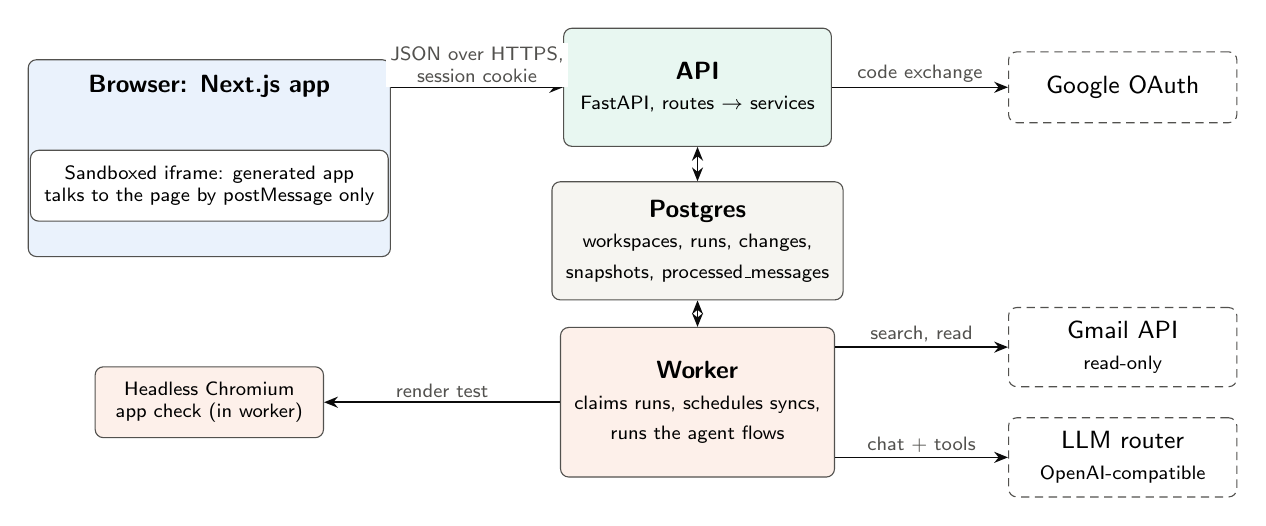
\begin{tikzpicture}[x=1cm,y=1cm]
% browser
\node[box,minimum width=4.6cm,minimum height=2.5cm,fill=bluebg] (web) at (0,0) {};
\node[font=\sffamily\small\bfseries,anchor=north] at ($(web.north)+(0,-0.08)$) {Browser: Next.js app};
\node[box,minimum width=4.0cm,fill=white,font=\sffamily\scriptsize] (frame) at (0,-0.35)
  {Sandboxed iframe: generated app\\talks to the page by postMessage only};
% api
\node[box,minimum width=3.4cm,minimum height=1.5cm,fill=aquabg] (api) at (6.2,0.9)
  {\textbf{API}\\{\scriptsize FastAPI, routes $\rightarrow$ services}};
% worker
\node[box,minimum width=3.4cm,minimum height=1.9cm,fill=orangebg] (worker) at (6.2,-3.1)
  {\textbf{Worker}\\{\scriptsize claims runs, schedules syncs,}\\{\scriptsize runs the agent flows}};
% db
\node[store,minimum width=3.4cm,minimum height=1.5cm] (db) at (6.2,-1.05)
  {\textbf{Postgres}\\{\scriptsize workspaces, runs, changes,}\\{\scriptsize snapshots, processed\_messages}};
% externals
\node[ext,minimum width=2.9cm] (google) at (11.6,0.9) {Google OAuth};
\node[ext,minimum width=2.9cm] (gmail) at (11.6,-2.4) {Gmail API\\{\scriptsize read-only}};
\node[ext,minimum width=2.9cm] (llm) at (11.6,-3.8) {LLM router\\{\scriptsize OpenAI-compatible}};
\node[box,minimum width=2.9cm,font=\sffamily\scriptsize,fill=orangebg] (chrome) at (0,-3.1)
  {Headless Chromium\\app check (in worker)};

\draw[flow] (web.east |- api.west) -- node[flowlab,above]{JSON over HTTPS,\\session cookie} (api.west);
\draw[flow,{Stealth[length=5pt,width=4pt]}-{Stealth[length=5pt,width=4pt]}] (api.south) -- (db.north);
\draw[flow,{Stealth[length=5pt,width=4pt]}-{Stealth[length=5pt,width=4pt]}] (worker.north) -- (db.south);
\draw[flow] (api.east) -- node[flowlab,above]{code exchange} (google.west);
\draw[flow] (worker.east |- gmail.west) -- node[flowlab,above]{search, read} (gmail.west);
\draw[flow] (worker.east |- llm.west) -- node[flowlab,above]{chat + tools} (llm.west);
\draw[flow] (worker.west) -- node[flowlab,above]{render test} (chrome.east);
\end{tikzpicture}
\caption{Processes and connections. Dashed boxes are external services. The API never calls
the LLM or Gmail; the worker never serves HTTP. They only share the database.}
\label{fig:arch}
\end{figure}

\begin{center}\small
\begin{tabularx}{\linewidth}{@{}P{2.5cm}P{4.4cm}L@{}}
\toprule
\textbf{Component} & \textbf{Code (under \code{backend/})} & \textbf{Responsibility} \\
\midrule
Web app & \file{../frontend/src} & Sign-in button, workspace list, the sandboxed app frame, activity feed, chat, undo, details drawer. Polls the API every 2\,s while a run is active, every 20\,s otherwise. \\
API & \file{app/api}, \file{app/services}, \file{app/auth} & Google OAuth, session cookie, workspace CRUD, enqueueing runs, undo, reading data and activity. Every query filters by \code{user\_id}. \\
Worker & \file{app/worker.py} & Claims queued runs, runs build / sync / edit, enqueues a sync for every ready workspace every 10 minutes. Up to 3 runs in parallel, one per workspace. \\
Agent & \file{app/agent} & The loop, the tools, the three flows, the prompts, the app check, the LLM client. Knows nothing about HTTP or SQL. \\
Mail & \file{app/mail} & The \code{Mailbox} interface (search, read thread) with a Gmail implementation and a fake one for tests, the CLI and the eval. \\
Store & \file{app/services/store.py} & Pure functions that validate and merge record saves, plus snapshots and undo. \\
\bottomrule
\end{tabularx}
\end{center}

\subsection{How the agent code is decoupled from the infrastructure}

The flows take a \code{RunContext} and a chat model, and nothing else. The context holds the
in-memory workspace state, a \code{Mailbox} and a \code{Persister}. Both are interfaces:

\begin{center}\small
\begin{tabularx}{\linewidth}{@{}P{3.0cm}P{4.6cm}L@{}}
\toprule
\textbf{Interface} & \textbf{Production} & \textbf{Tests, CLI, eval, benchmark} \\
\midrule
\code{Mailbox} & \code{GmailMailbox} (Gmail REST) & \code{FakeMailbox} (JSON file with a Gmail-like query matcher), \code{TimeBoxedMailbox} (hides mail after a date) \\
\code{Persister} & \code{DbPersister} (Postgres) & \code{MemoryPersister} (memory, optional folder) \\
\code{ChatModel} & \code{OpenAICompatibleLLM} & \code{ScriptedLLM} (replays fixed tool calls) \\
\bottomrule
\end{tabularx}
\end{center}

This is why the same \code{flows.build} runs in the worker, in \code{python -m app.agent.cli},
in the eval scenarios and in the benchmark of Section~\ref{sec:cost}, and why the 100 backend
tests need no network.

\subsection{Data model}

\begin{center}\small
\begin{tabularx}{\linewidth}{@{}P{3.2cm}L@{}}
\toprule
\textbf{Table} & \textbf{Contents} \\
\midrule
\code{users} & Google subject and email, Fernet-encrypted access and refresh tokens, \code{needs\_reconnect}. \\
\code{workspaces} & Prompt, status (\code{building}, \code{ready}, \code{failed}), queries, guide, data, app, version counters, \code{last\_synced\_at}, \code{last\_error}. At most 2 per user. \\
\code{runs} & One job: kind, status (\code{queued}, \code{running}, \code{done}, \code{failed}), input, progress events, summary, error, tokens and cost. This table is the queue. \\
\code{changes} & One row per record created, updated or deleted, with before and after values and source message ids. Feeds the Activity tab. \\
\code{snapshots} & The workspace state at the start of every run that may write. The newest 10 are kept. Feeds Undo. \\
\code{processed\_messages} & Which Gmail messages a workspace has already handled, so sync only reads new ones. \\
\bottomrule
\end{tabularx}
\end{center}

% =====================================================================
\section{The agent}

\subsection{One loop, four phases}

There is one agent loop (\file{agent/loop.py}, about 190 lines). It sends the conversation and
the tool schemas to the model, executes every tool call in the reply, appends the results, and
repeats until the phase is finished. What differs between phases is only the system prompt,
the set of tools and the step limit.

\begin{center}\small
\begin{tabularx}{\linewidth}{@{}P{1.5cm}P{3.5cm}P{1.3cm}L@{}}
\toprule
\textbf{Phase} & \textbf{Goal} & \textbf{Steps} & \textbf{Ends when} \\
\midrule
design & Write the guide and choose the queries & $\le 14$ & \code{finish} is called, or the guide and queries exist and the model stops calling tools \\
process & Turn one batch of threads into record saves & $\le 8$ & \code{finish}, or a second text-only reply \\
app & Write an app that passes the checks & $\le 6$ & \code{finish}, or the app is saved and the model stops \\
edit & Apply a chat request & $\le 30$ & \code{finish} \\
\bottomrule
\end{tabularx}
\end{center}

Loop rules that matter in practice:
\begin{itemize}
\item \textbf{Tool errors go back to the model} as \code{\{"error": ...\}} so it can correct itself. Three consecutive errors from the same tool fail the phase.
\item \textbf{A phase ends on its real goal}, not only on \code{finish}. Smaller models often answer in plain text when they are done; the loop accepts that once the phase's output exists.
\item \textbf{Old thread reads are dropped from the context}: only the 8 most recent \code{read\_thread} results are kept in full.
\item \textbf{Usage is recorded after every call}, and the persister raises when the run passes \usd{3} or the user passes \usd{15} for the day.
\end{itemize}

\subsection{Tools}

\begin{center}\small
\begin{tabularx}{\linewidth}{@{}P{2.7cm}cccc@{\hspace{8pt}}L@{}}
\toprule
\textbf{Tool} & \rotatebox{0}{\textbf{design}} & \textbf{process} & \textbf{app} & \textbf{edit} & \textbf{What it does and what it refuses} \\
\midrule
\code{search\_mail} & $\bullet$ & & & $\bullet$ & Gmail search inside the 90-day window. In design: at most 8 searches, 15 results each. \\
\code{read\_thread} & $\bullet$ & $\bullet$ & & $\bullet$ & Reads a thread the agent already knows. In design: at most 10 reads, 4 messages, 1,200 characters per body. \\
\code{read\_records} & & $\bullet$ & $\bullet$ & $\bullet$ & Returns current records (up to 200). \\
\code{save\_records} & & $\bullet$ & & $\bullet$ & Creates or merges records. Refuses a record that does not cite messages read in this run. \\
\code{delete\_records} & & $\bullet$ & & $\bullet$ & Deletes records. Requires a reason. \\
\code{write\_guide} & $\bullet$ & $\bullet$ & & $\bullet$ & Replaces the guide ($\le$ 6,000 characters). During sync only the ``Learned'' section may change. \\
\code{set\_queries} & $\bullet$ & & & $\bullet$ & Sets the queries and returns how many threads each matches. In design it refuses queries that match nothing. \\
\code{write\_app} & & & $\bullet$ & $\bullet$ & Checks the app statically and in a headless browser. Saves it only if it passes; otherwise returns the problems. \\
\code{request\_backfill} & & & & $\bullet$ & Asks for every known email to be re-read with the new guide after the edit. \\
\code{finish} & $\bullet$ & $\bullet$ & $\bullet$ & $\bullet$ & Ends the phase with a one-line summary. Refused in design before the guide and queries exist, and in app before the app is saved. \\
\bottomrule
\end{tabularx}
\end{center}

Every tool returns two things: the result for the model, and a short label for the progress
feed (``Saved 3 order records (2 new)''). Labels contain counts and type names only, never
email content, so they are safe to log and show.

\subsection{Guardrails enforced in code, not in the prompt}

The prompts state the rules, but the properties below hold even if the model ignores them.

\begin{center}\small
\begin{tabularx}{\linewidth}{@{}P{4.4cm}L@{}}
\toprule
\textbf{Property} & \textbf{Where it is enforced} \\
\midrule
No invented records & \code{apply\_save} rejects any record whose \code{source\_message\_ids} are not messages the agent received in this run. \\
Newer mail wins & Each record stores the date of its newest source. During a parallel backfill, a save from older mail may only fill empty fields. \\
Bounded data & At most 5 record types, 500 records, 20 fields per record, 2,000 characters per string. \\
Stable rule book during sync & \code{write\_guide} rejects changes above ``\# Learned'' in the process phase. \\
The app cannot reach the network or the page & Static rules and a headless render at write time; sandboxed iframe and CSP at display time (Section~\ref{sec:security}). \\
Bounded cost and time & Step limits, design budgets, batch size limits, per-run and per-day spending caps, 60\,s call timeout. \\
Every change is reversible & A snapshot is taken before every writing run; a failed edit restores it automatically. \\
\bottomrule
\end{tabularx}
\end{center}

% =====================================================================
\section{Sequences}

The diagrams read top to bottom. Solid arrows are calls, dashed arrows are returns or
asynchronous notifications.

\subsection{Sign-in}

The backend owns the whole OAuth flow. The browser only ever holds a signed session cookie;
Google tokens stay in the database, encrypted.

\begin{figure}[H]
\centering
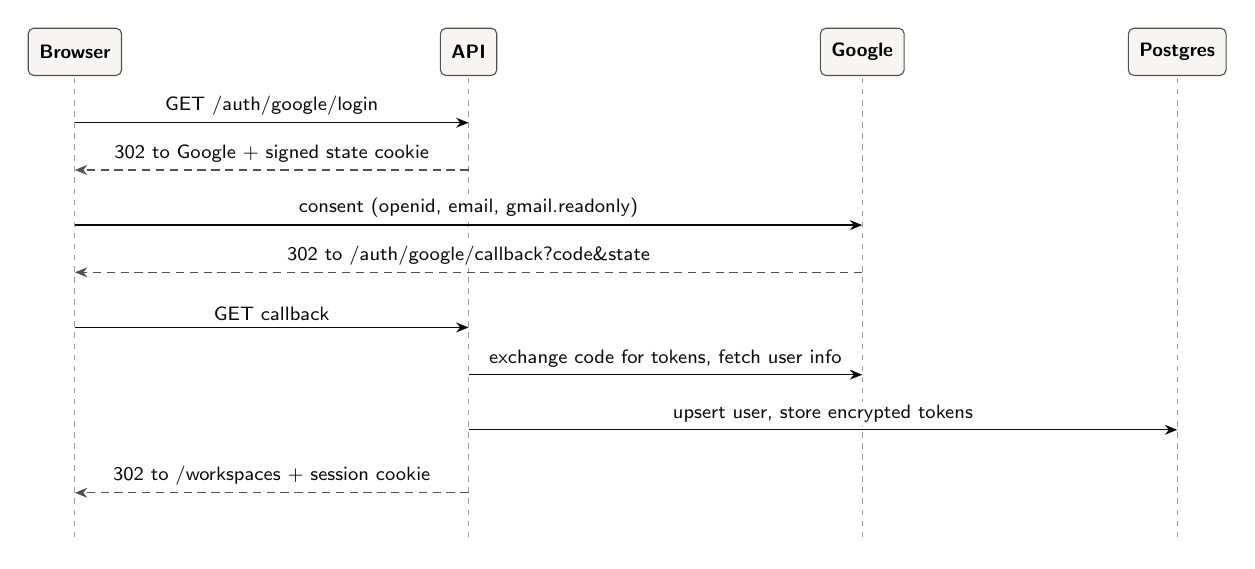
\begin{tikzpicture}[x=1cm,y=1cm]
\actor{u}{0}{Browser}{6.2}
\actor{a}{5}{API}{6.2}
\actor{g}{10}{Google}{6.2}
\actor{d}{14}{Postgres}{6.2}
\msg{u}{a}{0.9}{GET /auth/google/login}
\ret{a}{u}{1.5}{302 to Google + signed state cookie}
\msg{u}{g}{2.2}{consent (openid, email, gmail.readonly)}
\ret{g}{u}{2.8}{302 to /auth/google/callback?code\&state}
\msg{u}{a}{3.5}{GET callback}
\msg{a}{g}{4.1}{exchange code for tokens, fetch user info}
\msg{a}{d}{4.8}{upsert user, store encrypted tokens}
\ret{a}{u}{5.6}{302 to /workspaces + session cookie}
\end{tikzpicture}
\caption{Sign-in. The state cookie protects against cross-site request forgery. If Google later
rejects the refresh token, the user is flagged \code{needs\_reconnect}, syncing pauses and the
UI shows a ``Reconnect Gmail'' banner.}
\end{figure}

\subsection{Creating a workspace: from click to finished build}

The API only writes two rows and returns. All the work happens in the worker, and the browser
follows it by polling.

\begin{figure}[H]
\centering
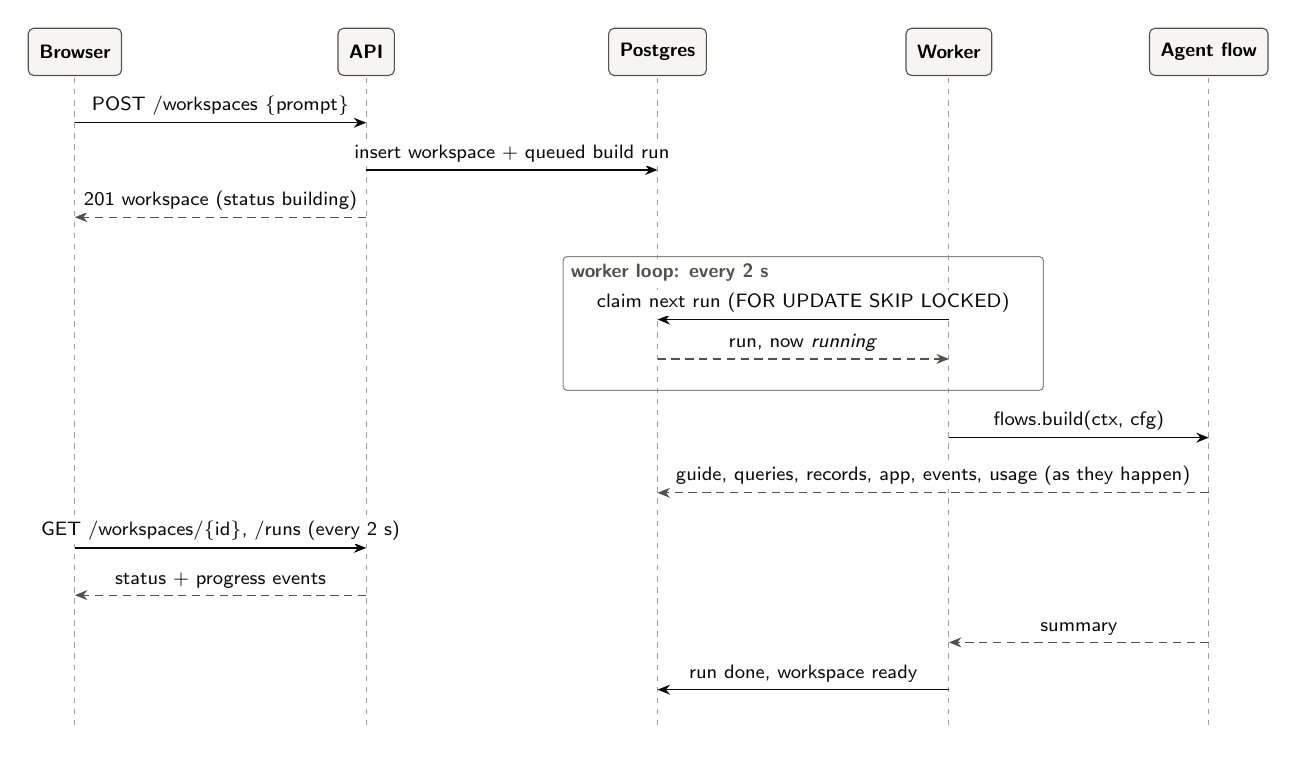
\begin{tikzpicture}[x=1cm,y=1cm]
\actor{u}{0}{Browser}{8.6}
\actor{a}{3.7}{API}{8.6}
\actor{d}{7.4}{Postgres}{8.6}
\actor{w}{11.1}{Worker}{8.6}
\actor{f}{14.4}{Agent flow}{8.6}
\msg{u}{a}{0.9}{POST /workspaces \{prompt\}}
\msg{a}{d}{1.5}{insert workspace + queued build run}
\ret{a}{u}{2.1}{201 workspace (status building)}
\frag{6.2}{2.6}{12.3}{4.3}{worker loop: every 2 s}
\msg{w}{d}{3.4}{claim next run (FOR UPDATE SKIP LOCKED)}
\ret{d}{w}{3.9}{run, now \emph{running}}
\msg{w}{f}{4.9}{flows.build(ctx, cfg)}
\ret{f}{d}{5.6}{guide, queries, records, app, events, usage (as they happen)}
\msg{u}{a}{6.3}{GET /workspaces/\{id\}, /runs (every 2 s)}
\ret{a}{u}{6.9}{status + progress events}
\ret{f}{w}{7.5}{summary}
\msg{w}{d}{8.1}{run done, workspace ready}
\end{tikzpicture}
\caption{Build as seen from outside the agent. A run is claimed only if its workspace has no
other running run, so two runs never write the same workspace at once.}
\end{figure}

\subsection{Inside a build}
\label{sec:build}

A build has three parts. The first is sequential; the second and third run at the same time,
which is what makes the build short.

Figure~\ref{fig:build} shows the calls. Details worth knowing:
\begin{itemize}
\item \textbf{Design works on a sample.} The model never sees the whole mailbox in one context. Its budgets (8 searches, 10 reads, 1,200 characters per body) keep the phase to a few seconds and a bounded number of tokens.
\item \textbf{The app is written from the guide, not from the data.} The guide lists the record types and fields, so the app can be written while the emails are still being read.
\item \textbf{Batches are independent.} Two batches can save the same record; stable ids make the saves merge, and the ``older mail only fills empty fields'' rule makes the result independent of which batch finishes first.
\item \textbf{A failed batch is retried once, then skipped} with a visible event. Its messages are still marked processed so a sync does not loop on them.
\item \textbf{Message bodies are cleaned} (HTML to text, quoted replies and signatures removed) and capped at 3,000 characters for new messages and 400 for context messages; a thread shows at most 10 messages.
\end{itemize}

\begin{figure}[H]
\centering
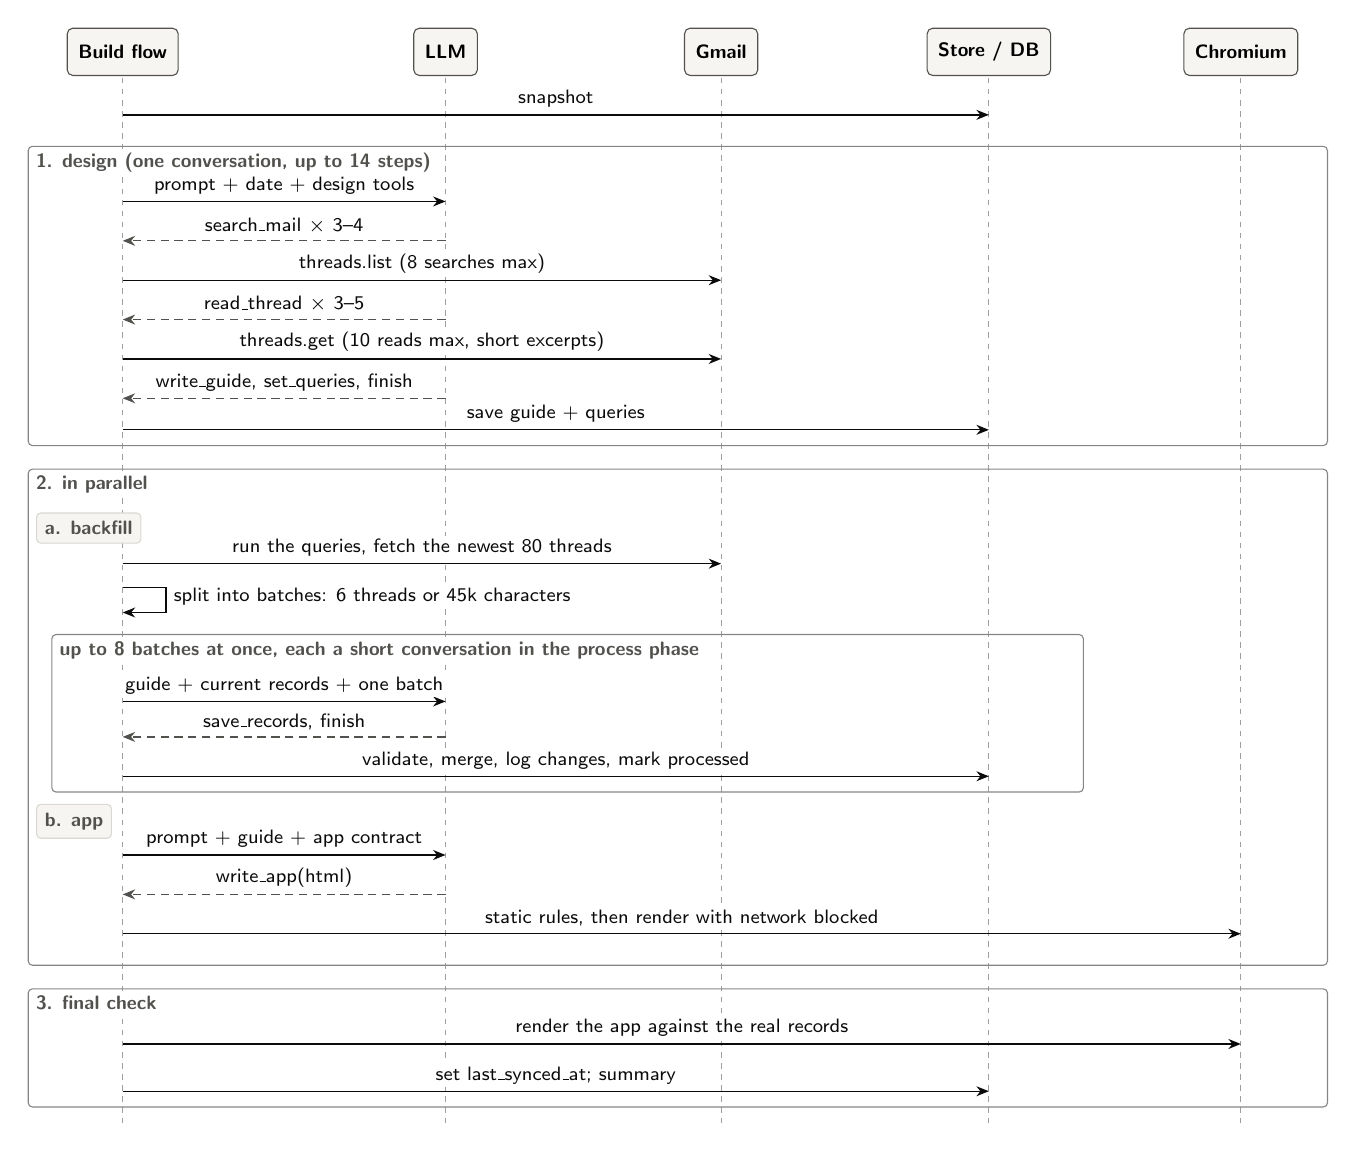
\begin{tikzpicture}[x=1cm,y=1cm]
\actor{f}{0}{Build flow}{13.6}
\actor{l}{4.1}{LLM}{13.6}
\actor{m}{7.6}{Gmail}{13.6}
\actor{s}{11.0}{Store / DB}{13.6}
\actor{c}{14.2}{Chromium}{13.6}

\msg{f}{s}{0.8}{snapshot}
\frag{-1.2}{1.2}{15.3}{5.0}{1. design (one conversation, up to 14 steps)}
\msg{f}{l}{1.9}{prompt + date + design tools}
\ret{l}{f}{2.4}{search\_mail $\times$ 3--4}
\msg{f}{m}{2.9}{threads.list (8 searches max)}
\ret{l}{f}{3.4}{read\_thread $\times$ 3--5}
\msg{f}{m}{3.9}{threads.get (10 reads max, short excerpts)}
\ret{l}{f}{4.4}{write\_guide, set\_queries, finish}
\msg{f}{s}{4.8}{save guide + queries}

\frag{-1.2}{5.3}{15.3}{11.6}{2. in parallel}
\node[note,anchor=north west] at (-1.1,-5.85) {\textbf{a. backfill}};
\msg{f}{m}{6.5}{run the queries, fetch the newest 80 threads}
\self{f}{6.8}{split into batches: 6 threads or 45k characters}
\frag{-0.9}{7.4}{12.2}{9.4}{up to 8 batches at once, each a short conversation in the process phase}
\msg{f}{l}{8.25}{guide + current records + one batch}
\ret{l}{f}{8.7}{save\_records, finish}
\msg{f}{s}{9.2}{validate, merge, log changes, mark processed}
\node[note,anchor=north west] at (-1.1,-9.55) {\textbf{b. app}};
\msg{f}{l}{10.2}{prompt + guide + app contract}
\ret{l}{f}{10.7}{write\_app(html)}
\msg{f}{c}{11.2}{static rules, then render with network blocked}

\frag{-1.2}{11.9}{15.3}{13.4}{3. final check}
\msg{f}{c}{12.6}{render the app against the real records}
\msg{f}{s}{13.2}{set last\_synced\_at; summary}
\end{tikzpicture}
\caption{Inside \code{flows.build}. Each batch is its own short conversation with the model, with
its own child context. If the final check fails, the app phase runs once more with the list of
problems; if that also fails, a built-in table view is used so the user always gets a working
interface.}
\label{fig:build}
\end{figure}

\subsection{Sync}

\begin{figure}[H]
\centering
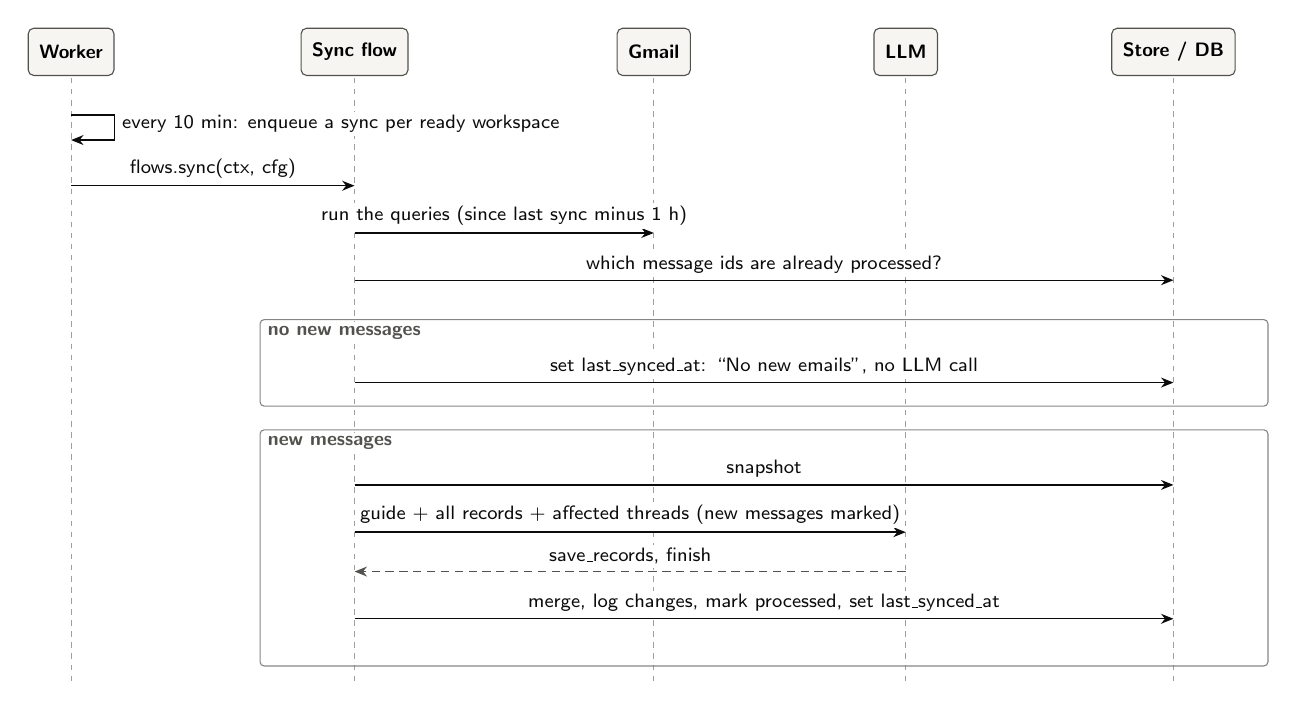
\begin{tikzpicture}[x=1cm,y=1cm]
\actor{w}{0}{Worker}{8.0}
\actor{f}{3.6}{Sync flow}{8.0}
\actor{m}{7.4}{Gmail}{8.0}
\actor{l}{10.6}{LLM}{8.0}
\actor{s}{14.0}{Store / DB}{8.0}
\self{w}{0.8}{every 10 min: enqueue a sync per ready workspace}
\msg{w}{f}{1.7}{flows.sync(ctx, cfg)}
\msg{f}{m}{2.3}{run the queries (since last sync minus 1 h)}
\msg{f}{s}{2.9}{which message ids are already processed?}
\frag{2.4}{3.4}{15.2}{4.5}{no new messages}
\msg{f}{s}{4.2}{set last\_synced\_at: ``No new emails'', no LLM call}
\frag{2.4}{4.8}{15.2}{7.8}{new messages}
\msg{f}{s}{5.5}{snapshot}
\msg{f}{l}{6.1}{guide + all records + affected threads (new messages marked)}
\ret{l}{f}{6.6}{save\_records, finish}
\msg{f}{s}{7.2}{merge, log changes, mark processed, set last\_synced\_at}
\end{tikzpicture}
\caption{Sync. Batches run one after another here, so each sees the data left by the previous
one. Runs that found nothing are pruned so the run list stays readable.}
\end{figure}

Two properties drive the running cost (Section~\ref{sec:upkeep}): a sync with no new matching
mail costs nothing, and a sync with new mail sends the guide and the current records along
with the new messages.

\subsection{Edit and undo}

\begin{figure}[H]
\centering
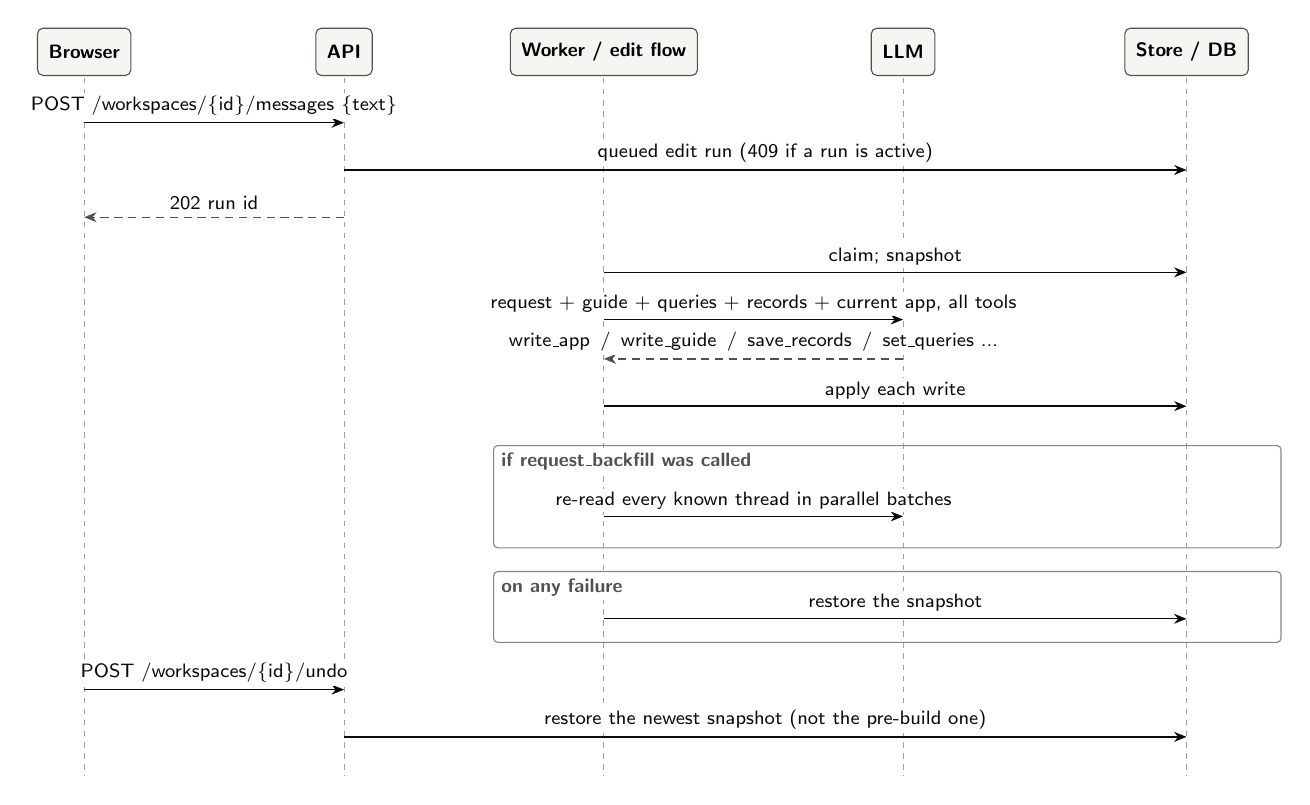
\begin{tikzpicture}[x=1cm,y=1cm]
\actor{u}{0}{Browser}{9.2}
\actor{a}{3.3}{API}{9.2}
\actor{w}{6.6}{Worker / edit flow}{9.2}
\actor{l}{10.4}{LLM}{9.2}
\actor{s}{14.0}{Store / DB}{9.2}
\msg{u}{a}{0.9}{POST /workspaces/\{id\}/messages \{text\}}
\msg{a}{s}{1.5}{queued edit run (409 if a run is active)}
\ret{a}{u}{2.1}{202 run id}
\msg{w}{s}{2.8}{claim; snapshot}
\msg{w}{l}{3.4}{request + guide + queries + records + current app, all tools}
\ret{l}{w}{3.9}{write\_app \,/\, write\_guide \,/\, save\_records \,/\, set\_queries ...}
\msg{w}{s}{4.5}{apply each write}
\frag{5.2}{5.0}{15.2}{6.3}{if request\_backfill was called}
\msg{w}{l}{5.9}{re-read every known thread in parallel batches}
\frag{5.2}{6.6}{15.2}{7.5}{on any failure}
\msg{w}{s}{7.2}{restore the snapshot}
\msg{u}{a}{8.1}{POST /workspaces/\{id\}/undo}
\msg{a}{s}{8.7}{restore the newest snapshot (not the pre-build one)}
\end{tikzpicture}
\caption{Edit and undo. Undo is a plain database restore handled by the API; no model is
involved.}
\end{figure}

\subsection{Showing the generated app}

The generated HTML is untrusted code. It runs in an iframe that has no origin, no network and
no access to the page, and exchanges data with the page only through messages.

\begin{figure}[H]
\centering
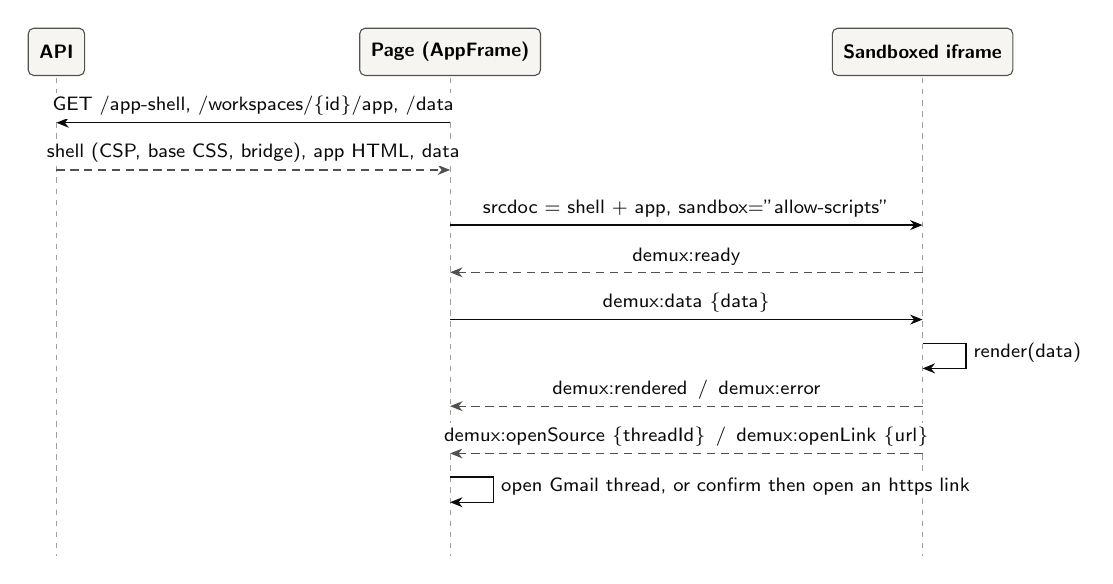
\begin{tikzpicture}[x=1cm,y=1cm]
\actor{a}{0}{API}{6.4}
\actor{p}{5}{Page (AppFrame)}{6.4}
\actor{i}{11}{Sandboxed iframe}{6.4}
\msg{p}{a}{0.9}{GET /app-shell, /workspaces/\{id\}/app, /data}
\ret{a}{p}{1.5}{shell (CSP, base CSS, bridge), app HTML, data}
\msg{p}{i}{2.2}{srcdoc = shell + app, sandbox="allow-scripts"}
\ret{i}{p}{2.8}{demux:ready}
\msg{p}{i}{3.4}{demux:data \{data\}}
\self{i}{3.7}{render(data)}
\ret{i}{p}{4.5}{demux:rendered \,/\, demux:error}
\ret{i}{p}{5.1}{demux:openSource \{threadId\} \,/\, demux:openLink \{url\}}
\self{p}{5.4}{open Gmail thread, or confirm then open an https link}
\end{tikzpicture}
\caption{Rendering. When the data version changes, the page posts \code{demux:data} again and
the app redraws without reloading. The same shell is used by the headless check in the worker,
so what passed the check is what the user sees.}
\end{figure}

% =====================================================================
\section{Security and privacy}
\label{sec:security}

\begin{center}\small
\begin{tabularx}{\linewidth}{@{}P{4.2cm}L@{}}
\toprule
\textbf{Risk} & \textbf{Control} \\
\midrule
Generated code steals data or calls out & Iframe with \code{sandbox="allow-scripts"} only (opaque origin, no cookies, no storage, no popups, no top navigation). CSP in the shell: \code{default-src 'none'}, inline script and style only, images and fonts from \code{data:} only. Static rules reject URLs, \code{fetch}, storage, \code{window.parent} and navigation before the app is saved. \\
An email tells the agent what to do & The prompts state that email content is data. More importantly, the agent has no tool that sends, deletes or shares anything: the worst an injected instruction can do is create a wrong record, which is logged and undoable. Scenario 07 of the eval tests this. \\
One user reads another's data & Every query filters by \code{user\_id}; a foreign workspace returns 404. \\
Google tokens leak & Tokens never leave the backend and are Fernet-encrypted at rest. The scope is \code{gmail.readonly}. \\
Email content in logs & Logs and progress events carry ids, counts, tool names and costs only. Debug transcripts are off by default and only available in development. \\
Runaway spending & \usd{3} per run and \usd{15} per user per day, checked after every model call. \\
\bottomrule
\end{tabularx}
\end{center}

% =====================================================================
\section{Reliability}

\begin{center}\small
\begin{tabularx}{\linewidth}{@{}P{4.2cm}L@{}}
\toprule
\textbf{Failure} & \textbf{What happens} \\
\midrule
Model call times out, 429 or 5xx & Up to 3 attempts on the main model, then up to 2 on the fallback model, with a short back-off. \\
Bad key, no credits, no permission (401, 402, 403) & Not retried. The run fails with a plain message telling the operator what to fix. \\
Model rejects \code{reasoning\_effort} & The parameter is dropped for that model and the call repeated. \\
Model ignores the tools or loops & Step limit per phase; three consecutive errors from one tool fail the phase with ``the agent could not finish this step''. \\
One batch fails twice & Skipped with a visible event; the rest of the build continues. \\
App never passes the checks & A built-in table view is used. The user can ask for another layout in chat. \\
Gmail rate limit (403) & Retried with back-off inside the Gmail client. \\
Gmail token revoked & User flagged for reconnect, syncs paused, banner in the UI. \\
Worker crashes mid-run & On restart, runs left \code{running} are marked failed (``Interrupted''). A failed build offers ``Try again''. \\
Edit fails half-way & The snapshot taken at the start is restored. \\
\bottomrule
\end{tabularx}
\end{center}

% =====================================================================
\section{Why a build is fast}

The first version of this build took 6.5 minutes on a real mailbox (and 13 minutes in one
test) before failing or finishing. The current one takes about 20 seconds. The changes, in order of effect:

\begin{enumerate}
\item \textbf{Parallel backfill.} Batches of threads are processed 8 at a time instead of one after another. This is safe because of the merge rules in the store, not because of the prompt.
\item \textbf{The app is written alongside the backfill}, from the guide.
\item \textbf{A bounded design phase.} An early real build read 58 threads during design and used 1.7 million input tokens. The budgets cap it at 10 short reads.
\item \textbf{A fast model without a thinking pass.} In one profiled build with thinking on, three design calls took 75 of 95 seconds (Section~\ref{sec:thinking}).
\item \textbf{A provider that accepts 8 parallel requests.} The same model on another provider rejected half of them with HTTP 429, and one test build took 199 seconds.
\item \textbf{A cap of 80 threads per build}, newest first.
\end{enumerate}

% =====================================================================
\section{Cost and response time}
\label{sec:cost}

\finding{\textbf{Summary.} Building a workspace costs \Nbuildlowcost{} for a low-volume
mailbox, \Nbuildmidcost{} for a mid-volume one and \Nbuildhighcost{} for a high-volume one.
Keeping it updated costs about \Nupkeeplow{}, \Nupkeepmid{} and \Nupkeephigh{} per month
respectively. The median build takes \Nlatmedian{} seconds; all \Nnbuilds{} completed builds finished in
under 30 seconds (slowest: \Nlatmax{} seconds). These are single-user figures on one provider
on one day.}

\subsection{How it was measured}
\label{sec:method}

The benchmark (\file{backend/eval/agent/bench}) runs the production flows with real model
calls against synthetic mailboxes, one run at a time, and records wall-clock time, tokens and
cost for every model call. It made \Nnruns{} runs and \Nllmcalls{} model calls for a total of
\Nbenchcost{}. A further \Nnnocredit{} runs at the very end were refused because the provider
account ran out of credits; they are excluded.

\begin{itemize}
\item \textbf{Three use cases}: online orders, supplier invoices, job applications. Each has its own prompt and its own mail.
\item \textbf{Three email volumes}, defined by how much relevant mail the last 90 days contain:
\end{itemize}

\begin{center}\small
\begin{tabularx}{0.92\linewidth}{@{}P{2.2cm}rrL@{}}
\toprule
\textbf{Volume} & \textbf{Threads to track} & \textbf{Other threads} & \textbf{Typical user} \\
\midrule
Low & 10 & 15 & A few orders or bills a month \\
Mid & 40 & 60 & Several relevant emails a week \\
High & 160 & 120 & Several a day; more than a build reads (the cap is 80 threads) \\
\bottomrule
\end{tabularx}
\end{center}

\begin{itemize}
\item \textbf{Mail that looks like real mail in size.} Threads have 1 to 3 messages. Message length is mixed: 30\% short (about 600 characters), 40\% medium (about 1,600) and 30\% long (3,200 to 4,200, above the pipeline's 3,000-character cap). Half of the ``other'' threads are promotions from the same senders, which the queries match and the agent must ignore.
\item \textbf{Three repeats} of every use case and volume (27 builds), plus builds of the eval scenarios (hand-written mailboxes of about 30 threads, each run up to twice), to widen the variety of prompts in the response-time distribution.
\item \textbf{Syncs} start from a finished build of every use case and volume and reveal 1, 3, 10 or 30 new emails: about half open new threads to track, about 30\% are follow-ups in existing threads, about 20\% are noise.
\item \textbf{Cost} is tokens multiplied by the list price of the measured model: \usd{0.45} per million input tokens and \usd{3.00} per million output tokens.
\item \textbf{Real Gmail}: the application database holds two builds, two syncs and one edit made on a real mailbox on the same day with the same configuration. Only their durations, token counts, costs and thread counts were read. They are shown next to the synthetic results as a check.
\end{itemize}

\subsection{Cost of building a workspace}

\begin{table}[H]
\centering\small
\begin{tabularx}{\linewidth}{@{}P{2.3cm}rrrrrrP{2.3cm}rP{1.6cm}@{}}
\toprule
& & \multicolumn{2}{c}{\textbf{Read}} & \multicolumn{2}{c}{\textbf{Tokens}} & \multicolumn{2}{c}{\textbf{Cost}} & \multicolumn{2}{c}{\textbf{Time}} \\
\cmidrule(lr){3-4}\cmidrule(lr){5-6}\cmidrule(lr){7-8}\cmidrule(l){9-10}
\textbf{Volume} & \textbf{n} & thr. & msg. & in & out & median & range & med. & range \\
\midrule
\tabin{generated/tab_build.tex}
\bottomrule
\end{tabularx}
\caption{Build cost and time. ``Read'' is the number of threads and messages the backfill
processed (medians). The number of threads read depends on the queries the model chooses: broad
queries also pull in threads that are then ignored.}
\label{tab:build}
\end{table}

\begin{figure}[H]
\centering
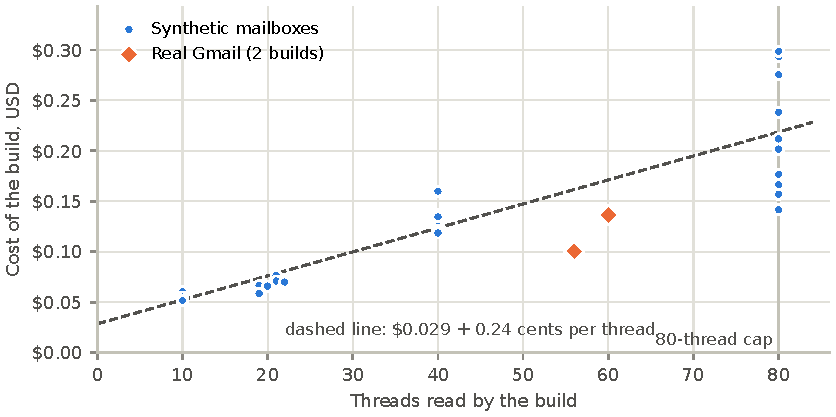
\includegraphics[width=0.86\linewidth]{figures/fig_cost_threads.pdf}
\caption{Build cost against the number of threads read. One dot per build.}
\label{fig:costthreads}
\end{figure}

Cost is close to linear in the number of threads read: a fixed part of about \Nfitfixed{}
(design and interface) plus about \Nfitperthreadcents{} cents per thread. Because a build reads
at most 80 threads, the fit puts a full build at about \Nfitcap{}. The two real Gmail builds
(56 and 60 threads, \usd{0.10} and \usd{0.14}) fall inside the synthetic cloud, which is the
main reason to trust the synthetic numbers.

\begin{figure}[H]
\centering
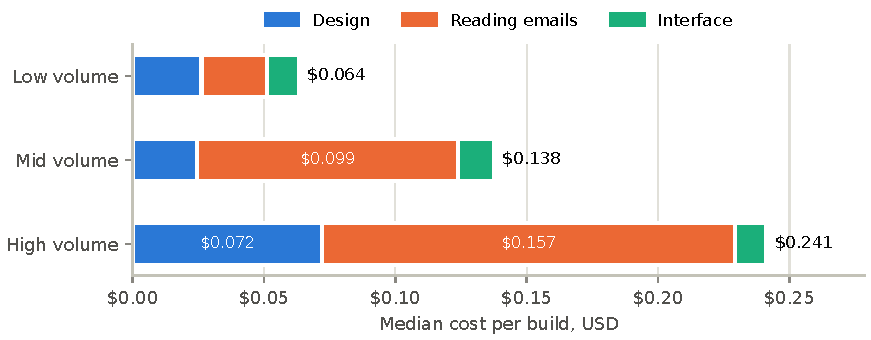
\includegraphics[width=0.86\linewidth]{figures/fig_phase_cost.pdf}
\caption{Where the money goes, by phase (median per build).}
\label{fig:phase}
\end{figure}

\begin{table}[H]
\centering\small
\begin{tabularx}{0.9\linewidth}{@{}P{1.6cm}LrLrLr@{}}
\toprule
& \multicolumn{2}{c}{\textbf{Design}} & \multicolumn{2}{c}{\textbf{Reading emails}} & \multicolumn{2}{c}{\textbf{Interface}} \\
\textbf{Volume} & cost (share) & calls & cost (share) & calls & cost (share) & calls \\
\midrule
\tabin{generated/tab_phase.tex}
\bottomrule
\end{tabularx}
\caption{Median cost and number of model calls per phase.}
\end{table}

What this means:
\begin{itemize}
\item \textbf{Design and interface are a floor} of about 4 cents per build. At low volume they are most of the bill. At high volume the design phase needed about twice as many calls (more search results to work through) and cost about 7 cents.
\item \textbf{Reading emails scales with volume} and dominates from mid volume upwards. Its cost is almost all input tokens: each batch sends the guide, the records saved so far and up to 6 threads.
\item \textbf{The worst case is bounded.} 80 threads of 10 messages at the 3,000-character cap would be far above anything measured, but a run stops at \usd{3} by configuration.
\end{itemize}

\subsection{Response time of workspace generation}

\begin{figure}[H]
\centering
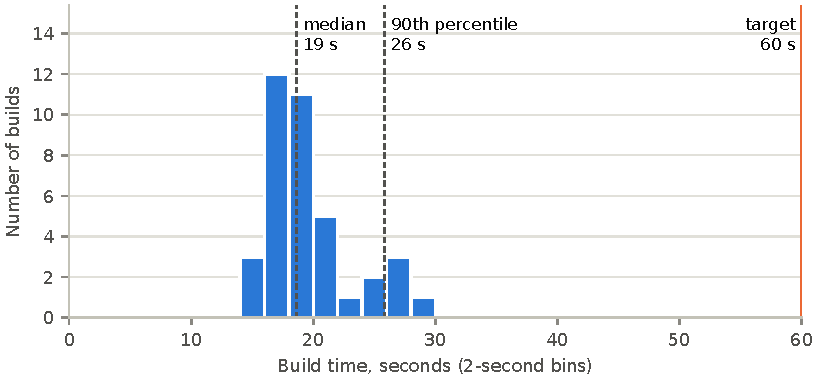
\includegraphics[width=0.86\linewidth]{figures/fig_latency_hist.pdf}
\caption{Distribution of build time over \Nnbuilds{} builds (27 on generated mailboxes, the rest
on eval scenarios), from the start of the run to the workspace being ready.}
\label{fig:lathist}
\end{figure}

\begin{table}[H]
\centering\small
\begin{tabularx}{0.86\linewidth}{@{}Lrrrrrrr@{}}
\toprule
\textbf{Builds} & \textbf{n} & \textbf{min} & \textbf{p10} & \textbf{median} & \textbf{p90} & \textbf{p95} & \textbf{max} \\
\midrule
\tabin{generated/tab_latency.tex}
\bottomrule
\end{tabularx}
\caption{Build time in seconds. Percentiles are interpolated; with these sample sizes p90 and
p95 are indicative only.}
\label{tab:latency}
\end{table}

\begin{figure}[H]
\centering
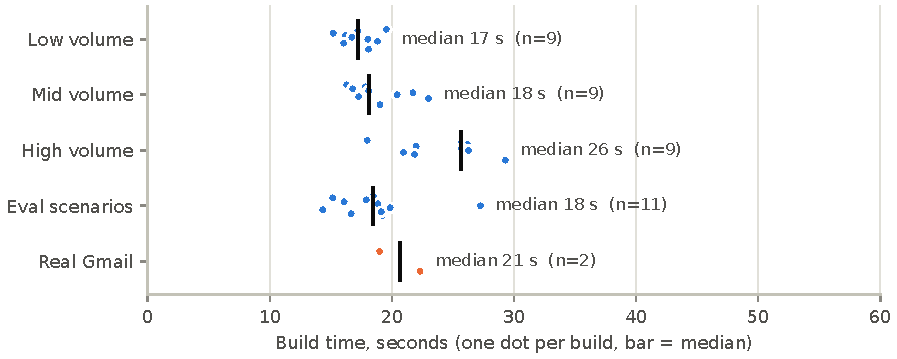
\includegraphics[width=0.86\linewidth]{figures/fig_latency_groups.pdf}
\caption{Build time by group, including the two real Gmail builds.}
\label{fig:latgroups}
\end{figure}

What this means:
\begin{itemize}
\item \textbf{Build time barely depends on email volume.} Batches are read in parallel, so 80 threads take little longer than 10. The fixed part is the design phase, which is sequential and takes about \Ndesignmedian{} seconds (about \Ndesignshare\% of a build).
\item \textbf{The target of one minute is met with margin} in this setting: all \Nnbuilds{} completed builds were under 30 seconds.
\item \textbf{What the user experiences adds up to 2 seconds of queue wait and up to 2 seconds of polling} on top of these figures, because the worker and the page both poll every 2 seconds.
\item \textbf{This distribution has no provider tail.} During the benchmark no model call had to be retried and none went to the fallback model. That is a good day, not a guarantee: each call may wait up to 60 seconds before it is retried, so on a bad provider day a build can take minutes. Earlier in the project, on other providers, builds took 199 and 398 seconds for exactly this reason.
\end{itemize}

Of the \Nnbuildsall{} builds started, \Nnbuildfail{} failed after 7 seconds: in eval scenario 07 the
model asked three times in a row to read a thread it had not found by search, and the loop
stopped the design phase. The user would see ``the agent could not finish this step'' and a
``Try again'' button. No build fell back to the built-in table view.

\subsection{Effect of the thinking pass}
\label{sec:thinking}

The model can be asked to reason before answering (\code{LLM\_REASONING\_EFFORT=low}). This
setting was not benchmarked: the provider account ran out of credits before the planned
comparison could run. The only evidence is two test builds of eval scenario 04 made with
thinking on before the benchmark, against the benchmark's builds of the same scenario with
thinking off.

\begin{table}[H]
\centering\small
\begin{tabularx}{0.8\linewidth}{@{}Lrrrr@{}}
\toprule
\textbf{Scenario 04 build} & \textbf{n} & \textbf{Time} & \textbf{Cost} & \textbf{Output tokens} \\
\midrule
Thinking off (default) & 2 & 18\,s, 19\,s & \$0.07, \$0.09 & 7.6k, 10k \\
Thinking on, low effort & 2 & 55\,s, 96\,s & \$0.12, \$0.20 & 28k, 50k \\
\bottomrule
\end{tabularx}
\caption{Thinking on and off, same scenario. Four builds: an indication, not a measurement.}
\end{table}

In the slower of the two thinking builds, three design calls produced about 16,000 output
tokens each and took 76 of the 96 seconds. Output tokens are both the expensive ones and the
slow ones, and a thinking pass multiplies them. Whether better records are worth it is a
product decision that needs a proper comparison, with the eval suite measuring the quality
side.

\subsection{Cost of keeping a workspace updated}
\label{sec:upkeep}

A sync that finds no new matching mail makes no model call and costs nothing. A sync with new
mail makes one short conversation per batch of threads.

\begin{table}[H]
\centering\small
\begin{tabularx}{\linewidth}{@{}P{1.5cm}r@{\hspace{14pt}}rrrrrrrr@{}}
\toprule
& & \multicolumn{2}{c}{\textbf{1 new email}} & \multicolumn{2}{c}{\textbf{3 new}} & \multicolumn{2}{c}{\textbf{10 new}} & \multicolumn{2}{c}{\textbf{30 new}} \\
\cmidrule(lr){3-4}\cmidrule(lr){5-6}\cmidrule(lr){7-8}\cmidrule(l){9-10}
\textbf{Workspace} & \textbf{Records} & cost & time & cost & time & cost & time & cost & time \\
\midrule
\tabin{generated/tab_sync.tex}
\bottomrule
\end{tabularx}
\caption{Cost and time of one sync (medians), by the size of the workspace it updates and the
number of new emails it finds.}
\label{tab:sync}
\end{table}

\begin{figure}[H]
\centering
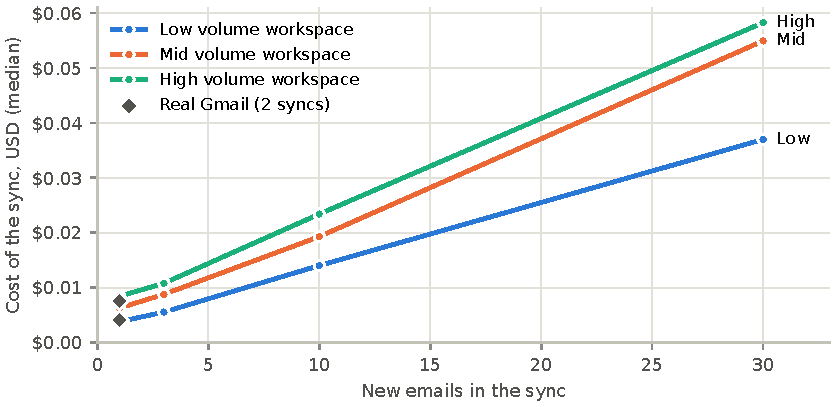
\includegraphics[width=0.86\linewidth]{figures/fig_sync_cost.pdf}
\caption{Sync cost against the number of new emails.}
\label{fig:sync}
\end{figure}

A sync has a fixed part and a part per email. The fixed part grows with the workspace, because
the guide and the current records are sent with every batch: it is \Nsyncfixedlow{} for a
low-volume workspace and \Nsyncfixedhigh{} for a high-volume one. The real Gmail syncs (1 new
email each, \usd{0.004} and \usd{0.008}) are in the same range.

The monthly cost then depends on how many new emails match the queries per day and on how they
are spread over the day. Table~\ref{tab:upkeep} assumes emails arrive at random times, so
several can land in the same 10-minute sync.

\begin{table}[H]
\centering\small
\begin{tabularx}{\linewidth}{@{}Lrrrrrrr@{}}
\toprule
& \textbf{New emails} & & \textbf{Fixed} & \textbf{Per} & \textbf{Syncs with} & \textbf{Estimate} & \\
\textbf{Volume} & \textbf{per day} & \textbf{Records} & \textbf{per sync} & \textbf{email} & \textbf{mail per day} & \textbf{per month} & \textbf{Range} \\
\midrule
\tabin{generated/tab_upkeep.tex}
\bottomrule
\end{tabularx}
\caption{Monthly cost of keeping one workspace updated. ``Fixed per sync'' and ``per email'' are
a straight-line fit to the measured syncs of that workspace size. The range runs from all of a
day's emails arriving together to every email arriving in its own sync.}
\label{tab:upkeep}
\end{table}

Three cautions on these estimates:
\begin{itemize}
\item \textbf{``New emails'' means emails matching the queries}, including promotions and other noise the agent then ignores. The queries are deliberately broad, so this number is higher than the number of emails the user cares about.
\item \textbf{The fixed part grows as the workspace fills up.} A workspace that keeps adding records for months moves towards the high-volume line, up to the 500-record limit.
\item \textbf{The 144 automatic syncs per day that find nothing are free in model cost}, but each makes one Gmail search per query.
\end{itemize}

\subsection{Other operations}

\begin{table}[H]
\centering\small
\begin{tabularx}{0.92\linewidth}{@{}Lrrrrr@{}}
\toprule
\textbf{Operation} & \textbf{n} & \textbf{Median cost} & \textbf{Range} & \textbf{Median time} & \textbf{Range} \\
\midrule
\tabin{generated/tab_other.tex}
\bottomrule
\end{tabularx}
\caption{Edits and syncs measured on the eval scenarios, with the real Gmail runs for
comparison.}
\end{table}

\subsection{Final estimates}

\begin{center}\small\renewcommand{\arraystretch}{1.35}
\begin{tabularx}{\linewidth}{@{}P{5.2cm}LLL@{}}
\toprule
& \textbf{Low volume} & \textbf{Mid volume} & \textbf{High volume} \\
\midrule
Build a workspace (one-off) & \$0.066 & \$0.14 & \$0.24 \\
Keep it updated (per month) & \$0.20 & \$1.66 & \$10.1 \\
Build time (median) & 17\,s & 18\,s & 26\,s \\
\bottomrule
\end{tabularx}\end{center}


\begin{itemize}
\item \textbf{Per user, first month}: one build plus one month of upkeep per workspace, so roughly \Nbuildlowcost{} + \Nupkeeplow{} at low volume and \Nbuildhighcost{} + \Nupkeephigh{} at high volume, before any chat edits (2 to 6 cents each in the few measured).
\item \textbf{The steady-state cost is the upkeep}, not the build. At high volume one month of syncing costs many times the build.
\item \textbf{These figures scale with the model's price.} A model that costs five times more per token costs about five times more here, and one with a thinking pass more than that. They are specific to \code{Qwen/Qwen3.8-27B} on Nebius at November 2026 list prices.
\item \textbf{The cheapest lever on upkeep} is to stop sending all records with every sync (send only the records that the new threads could match), which would remove most of the fixed part at high volume. This has not been built.
\end{itemize}


% =====================================================================
\section{Quality snapshot and known limits}
\label{sec:limits}

\subsection{Extraction quality with the current model}

The eval suite (\code{make eval-agent}) runs 8 synthetic scenarios, each with a build, a sync
and an edit, and checks 155 expectations. On 16 November 2026 the current configuration passed
121 of them (78\%), in one run. Scenarios 01, 03, 07 and 08 passed every check, scenario 04
passed 28 of 30 and scenario 06 passed 13 of 18. The two weak ones were scenario 02 (10 of 23)
and scenario 05 (13 of 27), where the model created duplicate records for the same real-world
thing and missed some status updates. One run
is not enough to rank changes: the suite should be run with \code{--repeats 3} before any
decision that depends on a few points.

Speed was bought with quality. Turning the thinking pass off and using a 27B model makes the
build about 20 seconds and about 10 cents, but a stronger model produces better records. The
model is one line of configuration, and build and sync models are separate settings, so a
stronger model for build with a cheap one for sync is a possible middle ground that this report
did not measure.

\subsection{What the numbers in this report do not cover}

\begin{itemize}
\item \textbf{Real Gmail at volume.} Only two real builds and two real syncs were available. They agree with the synthetic results, but two points are not a distribution.
\item \textbf{Several users at once.} The benchmark ran one build at a time. With many builds running together, provider rate limits and the worker's limit of 3 parallel runs will add waiting time.
\item \textbf{The thinking pass.} The planned comparison did not run because the provider account ran out of credits (Section~\ref{sec:thinking}).
\item \textbf{Provider drift.} Prices and speed of hosted open models change, sometimes within a day. During this project three providers failed in three different ways (HTTP 500s, exhausted credits, rate limits).
\item \textbf{Mail that does not look like the test mail.} Very long threads, non-English mail and attachments-only mail were not measured. Attachments are listed by name but never read.
\item \textbf{Workspaces larger than a few hundred records.} The current records are sent with every sync; near the 500-record limit this dominates the sync cost.
\end{itemize}

\subsection{Design limits to keep in mind}

\begin{itemize}
\item A build reads at most 80 threads from the last 90 days. Older or additional mail is not picked up later unless the queries change.
\item The run queue is a Postgres table polled every 2 seconds by a single worker process. That is enough for a trial; it is not a scaling design.
\item The frontend polls; there is no push channel.
\item Each user is limited to 2 workspaces.
\end{itemize}

% =====================================================================
\appendix
\section{Configuration reference}

All settings live in the repository-root \code{.env} and are read by
\file{backend/app/core/config.py}.

\begin{center}\small
\begin{tabularx}{\linewidth}{@{}P{4.6cm}P{4.4cm}L@{}}
\toprule
\textbf{Setting} & \textbf{Default} & \textbf{Effect} \\
\midrule
\code{BUILD\_MODEL} & \code{Qwen/Qwen3.8-27B:nebius} & Design, app and edit phases \\
\code{SYNC\_MODEL} & \code{Qwen/Qwen3.8-27B:nebius} & Process phase (backfill and sync) \\
\code{LLM\_FALLBACK\_MODEL} & \code{Qwen/Qwen3.8-27B:nscale} & Used after 3 failed attempts \\
\code{LLM\_REASONING\_EFFORT} & \code{none} & Thinking pass; \code{low} is slower and better \\
\code{LLM\_MAX\_TOKENS} & 8000 & Output cap per call \\
\code{LLM\_CALL\_TIMEOUT\_S} & 60 & Per call \\
\code{BUILD\_MAX\_THREADS} & 80 & Threads read by a build \\
\code{BATCH\_THREADS}, \code{BATCH\_MAX\_CHARS} & 6, 45000 & Batch size limits \\
\code{PROCESS\_CONCURRENCY} & 8 & Parallel batches in a backfill \\
\code{LOOKBACK\_DAYS} & 90 & Mail window \\
\code{SYNC\_INTERVAL\_MIN} & 10 & Automatic sync period \\
\code{MAX\_USD\_PER\_RUN}, \code{MAX\_USD\_PER\_DAY} & 3, 15 & Spending caps \\
\code{WORKER\_CONCURRENCY} & 3 & Runs in parallel \\
\bottomrule
\end{tabularx}
\end{center}

Prices used for cost accounting are in \file{backend/app/agent/prices.yaml}. For the measured
model they are \usd{0.45} per million input tokens and \usd{3.00} per million output tokens.

\section{Where things are}

\begin{center}\small
\begin{tabularx}{\linewidth}{@{}P{5.6cm}L@{}}
\toprule
\textbf{Path (under \code{backend/})} & \textbf{Contents} \\
\midrule
\file{app/agent/loop.py} & The agent loop \\
\file{app/agent/flows.py} & Build, sync, edit; batching and parallelism \\
\file{app/agent/tools.py} & Tool schemas and implementations, phase-to-tool map \\
\file{app/agent/prompts.py} & System prompts and input builders \\
\file{app/agent/llm.py}, \file{prices.yaml} & LLM client, retries, fallback, cost \\
\file{app/agent/appcheck.py}, \file{shell.py} & App checks; CSP, base CSS and bridge \\
\file{app/agent/context.py} & \code{RunContext}, \code{Persister}, \code{MemoryPersister} \\
\file{app/services/store.py} & Record validation and merge, snapshots, undo \\
\file{app/services/runs.py} & Queue, claiming, \code{DbPersister}, budgets \\
\file{app/worker.py} & Worker process \\
\file{app/mail/} & Mailbox interface, Gmail client, fake mailbox, cleaning \\
\file{app/auth/}, \file{app/api/routes/} & OAuth, session, HTTP routes \\
\file{eval/agent/} & Scenarios, runner, scoring, replay \\
\file{eval/agent/bench/} & The benchmark behind Section~\ref{sec:cost} \\
\file{tests/} & 100 tests, no network needed \\
\bottomrule
\end{tabularx}
\end{center}

\section{Reproducing the measurements}

\begin{verbatim}
cd backend
uv run python -m eval.agent.bench --repeats 3        # builds, syncs, scenarios
uv run --with matplotlib python ../docs/report/analyze.py \
       eval/agent/runs/bench-main/results.jsonl      # figures and tables
\end{verbatim}

The benchmark makes real model calls (\Nbenchcost{} in total for the main run reported here) against synthetic mailboxes generated by \file{mailgen.py} in the same folder. The results
file is copied to \file{docs/report/data/}.

\end{document}
